\documentclass[a4paper,12pt]{article}

\usepackage[utf8x]{inputenc}
\usepackage[T2A]{fontenc}
\usepackage[english, russian]{babel}

% Опционно, требует  apt-get install scalable-cyrfonts.*
% и удаления одной строчки в cyrtimes.sty
% Сточку не удалять!
% \usepackage{cyrtimes}

% Картнки и tikz
\usepackage{graphicx}
\usepackage{tikz}
\usetikzlibrary{snakes,arrows,shapes}


% Некоторая русификация.
\usepackage{misccorr}
\usepackage{indentfirst}
\renewcommand{\labelitemi}{\normalfont\bfseries{--}}

% Увы, поля придётся уменьшить из-за листингов.
\topmargin -1cm
\oddsidemargin -0.5cm
\evensidemargin -0.5cm
\textwidth 17cm
\textheight 24cm

\sloppy

% Оглавление в PDF
\usepackage[
bookmarks=true,
colorlinks=true, linkcolor=black, anchorcolor=black, citecolor=black, menucolor=black,filecolor=black, urlcolor=black,
unicode=true
]{hyperref}

% Для исходного кода в тексте
\newcommand{\Code}[1]{\textbf{#1}}

\usepackage{verbatim}
\usepackage{fancyvrb}
\fvset{frame=leftline, fontsize=\small, framerule=0.4mm, rulecolor=\color{darkgray}, commandchars=\\\{\}}
\renewcommand{\theFancyVerbLine}{\small\arabic{FancyVerbLine}}



\title{Отчёт по лабораторной работе \\ <<Система доменных имён>>}
\author{Пучниной Анастасии Ивановны}

\begin{document}

\maketitle

\tableofcontents

\section{Настройка системы DNS}

\subsection{Топология сети}

Топология сети и использыемые IP-адреса показаны на рис.~\ref{fig:network}.

\begin{figure}
\centering
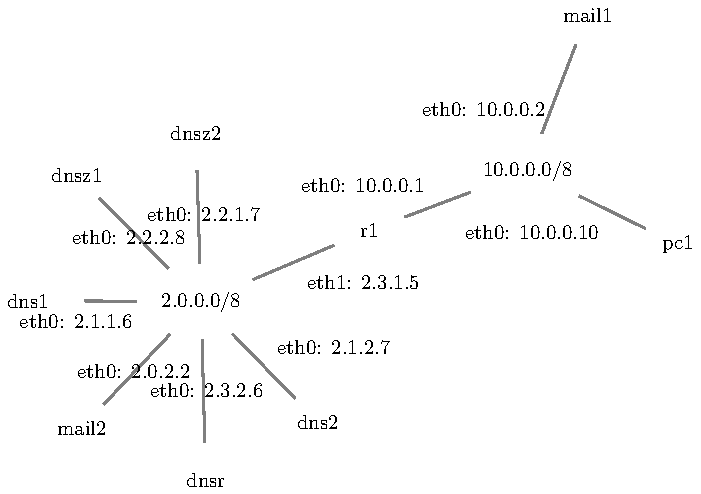
\includegraphics[width=\textwidth]{includes/network_gv.pdf}
\caption{Топология сети}
\label{fig:network}
\end{figure}

\subsection{Структура службы доменных имён}

Структура авторитетных серверов доменных имён показана на рис.~\ref{fig:dns}.

\begin{figure}
\centering
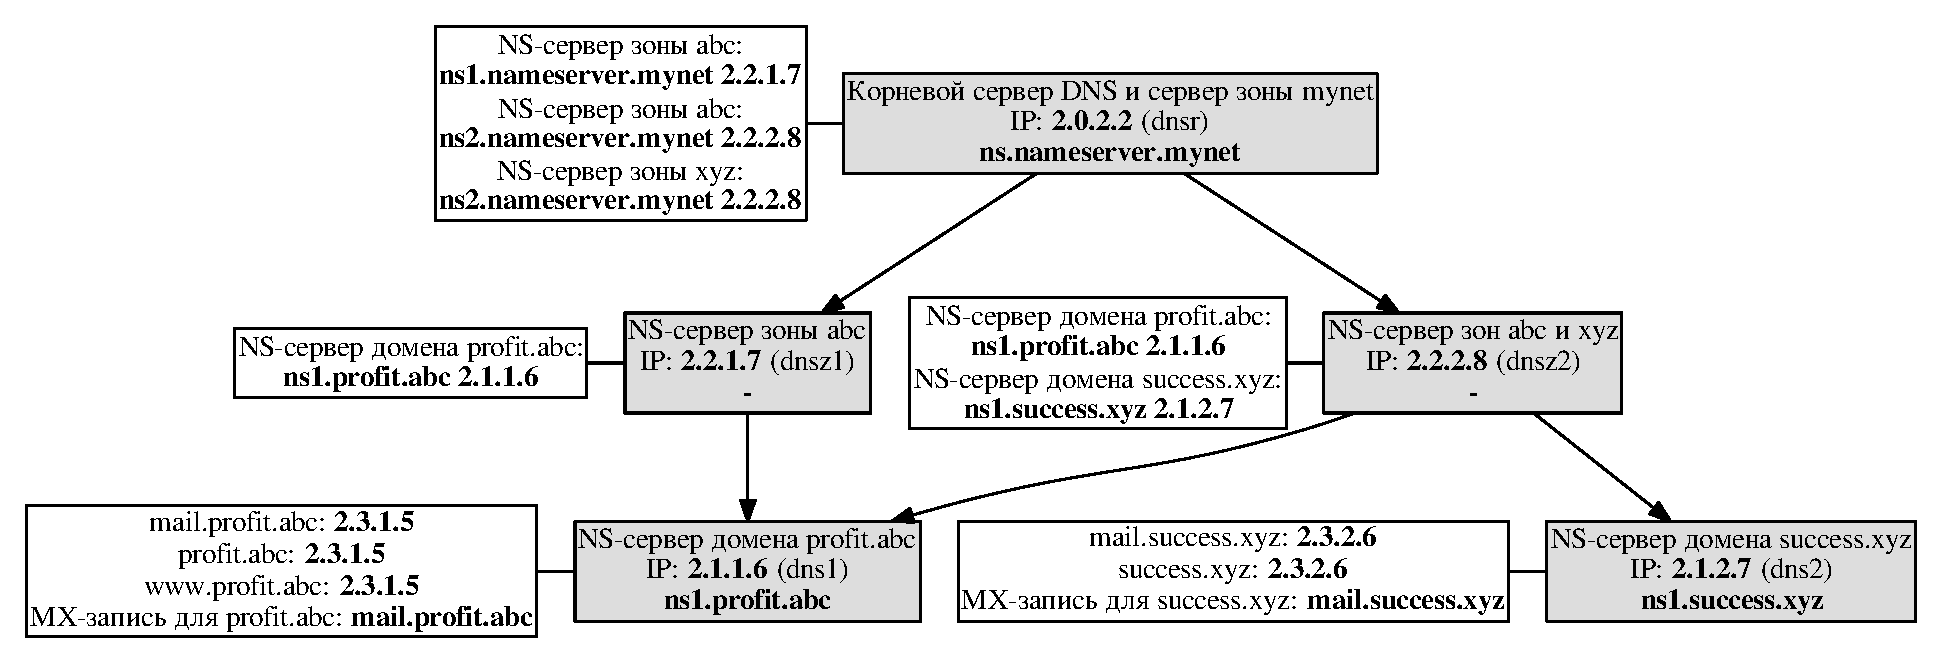
\includegraphics[width=\textwidth]{includes/dns_gv.pdf}
\caption{Структура службы доменных имён}
\label{fig:dns}
\end{figure}

\subsection{Прочие настройки}

Кеширующие DNS-серверы
\begin{itemize}
\item ... ;
\item ...
\end{itemize}

Развёрнутые SMTP-серверы и используемые ими кеширующие DNS-серверы.
\begin{itemize}
\item ... использует сервер на ... ;
\item ...
\end{itemize}


\section{Проверка настройки службы доменных имён}

\subsection{Проверка настройки записи типа MX для домена profit.abc}

По цепочке опрашиваем с корневого сервера:

\begin{verbatim}
mail2:~# dig @2.0.2.2 profit.abc MX

; <<>> DiG 9.5.0-P2 <<>> @2.0.2.2 profit.abc MX
; (1 server found)
;; global options:  printcmd
;; Got answer:
;; ->>HEADER<<- opcode: QUERY, status: NOERROR, id: 25690
;; flags: qr rd; QUERY: 1, ANSWER: 0, AUTHORITY: 2, ADDITIONAL: 2
;; WARNING: recursion requested but not available

;; QUESTION SECTION:
;profit.abc.			IN	MX

;; AUTHORITY SECTION:
abc.			86400	IN	NS	ns1.nameserver.mynet.
abc.			86400	IN	NS	ns2.nameserver.mynet.

;; ADDITIONAL SECTION:
ns1.nameserver.mynet.	86400	IN	A	2.2.1.7
ns2.nameserver.mynet.	86400	IN	A	2.2.2.8

;; Query time: 3 msec
;; SERVER: 2.0.2.2#53(2.0.2.2)
;; WHEN: Sat Dec 15 03:22:59 2018
;; MSG SIZE  rcvd: 112

\end{verbatim}

Опрашиваем следующий сервер abc. по одному из полученных адресов (2.2.1.7):

\begin{verbatim}
mail2:~# dig @2.2.1.7 profit.abc MX

; <<>> DiG 9.5.0-P2 <<>> @2.2.1.7 profit.abc MX
; (1 server found)
;; global options:  printcmd
;; Got answer:
;; ->>HEADER<<- opcode: QUERY, status: NOERROR, id: 44926
;; flags: qr rd; QUERY: 1, ANSWER: 0, AUTHORITY: 1, ADDITIONAL: 1
;; WARNING: recursion requested but not available

;; QUESTION SECTION:
;profit.abc.			IN	MX

;; AUTHORITY SECTION:
profit.abc.		86400	IN	NS	ns1.profit.abc.

;; ADDITIONAL SECTION:
ns1.profit.abc.		86400	IN	A	2.1.1.6

;; Query time: 5 msec
;; SERVER: 2.2.1.7#53(2.2.1.7)
;; WHEN: Sat Dec 15 03:24:05 2018
;; MSG SIZE  rcvd: 62
\end{verbatim}

Опрашиваем следующий NS-сервер profit.abc. с адресом 2.1.1.6:

\begin{verbatim}
mail2:~# dig @2.1.1.6 profit.abc MX

; <<>> DiG 9.5.0-P2 <<>> @2.1.1.6 profit.abc MX
; (1 server found)
;; global options:  printcmd
;; Got answer:
;; ->>HEADER<<- opcode: QUERY, status: NOERROR, id: 59319
;; flags: qr aa rd; QUERY: 1, ANSWER: 1, AUTHORITY: 1, ADDITIONAL: 2
;; WARNING: recursion requested but not available

;; QUESTION SECTION:
;profit.abc.			IN	MX

;; ANSWER SECTION:
profit.abc.		86400	IN	MX	10 mail.profit.abc.

;; AUTHORITY SECTION:
profit.abc.		86400	IN	NS	ns1.profit.abc.

;; ADDITIONAL SECTION:
mail.profit.abc.	86400	IN	A	2.3.1.5
ns1.profit.abc.		86400	IN	A	2.1.1.6

;; Query time: 8 msec
;; SERVER: 2.1.1.6#53(2.1.1.6)
;; WHEN: Sat Dec 15 03:24:50 2018
;; MSG SIZE  rcvd: 99
\end{verbatim}

Итоговая проверка: опрашиваем кеширующий DNS-сервер.

\begin{verbatim}
pc1:~# dig @10.0.0.1 profit.abc MX

; <<>> DiG 9.5.0-P2 <<>> @10.0.0.1 profit.abc MX
; (1 server found)
;; global options:  printcmd
;; Got answer:
;; ->>HEADER<<- opcode: QUERY, status: NOERROR, id: 32294
;; flags: qr rd ra; QUERY: 1, ANSWER: 1, AUTHORITY: 0, ADDITIONAL: 1

;; QUESTION SECTION:
;profit.abc.			IN	MX

;; ANSWER SECTION:
profit.abc.		86390	IN	MX	10 mail.profit.abc.

;; ADDITIONAL SECTION:
mail.profit.abc.	86390	IN	A	2.3.1.5

;; Query time: 4 msec
;; SERVER: 10.0.0.1#53(10.0.0.1)
;; WHEN: Sat Dec 15 03:33:05 2018
;; MSG SIZE  rcvd: 65

\end{verbatim}

\begin{verbatim}
pc1:~# ping profit.abc
PING profit.abc (2.3.1.5) 56(84) bytes of data.
64 bytes from 2.3.1.5: icmp_seq=1 ttl=64 time=0.175 ms
64 bytes from 2.3.1.5: icmp_seq=2 ttl=64 time=0.509 ms
^C
--- profit.abc ping statistics ---
2 packets transmitted, 2 received, 0% packet loss, time 1014ms
rtt min/avg/max/mdev = 0.175/0.342/0.509/0.167 ms
\end{verbatim}

\subsection{Проверка настройки записи типа A для домена success.xyz}

\begin{verbatim}
mail2:~# dig @2.0.2.2 success.xyz A

; <<>> DiG 9.5.0-P2 <<>> @2.0.2.2 success.xyz A
; (1 server found)
;; global options:  printcmd
;; Got answer:
;; ->>HEADER<<- opcode: QUERY, status: NOERROR, id: 2901
;; flags: qr rd; QUERY: 1, ANSWER: 0, AUTHORITY: 1, ADDITIONAL: 1
;; WARNING: recursion requested but not available

;; QUESTION SECTION:
;success.xyz.			IN	A

;; AUTHORITY SECTION:
xyz.			86400	IN	NS	ns2.nameserver.mynet.

;; ADDITIONAL SECTION:
ns2.nameserver.mynet.	86400	IN	A	2.2.2.8

;; Query time: 3 msec
;; SERVER: 2.0.2.2#53(2.0.2.2)
;; WHEN: Sat Dec 15 03:37:02 2018
;; MSG SIZE  rcvd: 79

\end{verbatim}

\begin{verbatim}
mail2:~# dig @2.2.2.8 success.xyz A

; <<>> DiG 9.5.0-P2 <<>> @2.2.2.8 success.xyz A
; (1 server found)
;; global options:  printcmd
;; Got answer:
;; ->>HEADER<<- opcode: QUERY, status: NOERROR, id: 62523
;; flags: qr rd; QUERY: 1, ANSWER: 0, AUTHORITY: 1, ADDITIONAL: 1
;; WARNING: recursion requested but not available

;; QUESTION SECTION:
;success.xyz.			IN	A

;; AUTHORITY SECTION:
success.xyz.		86400	IN	NS	ns1.success.xyz.

;; ADDITIONAL SECTION:
ns1.success.xyz.	86400	IN	A	2.1.2.7

;; Query time: 20 msec
;; SERVER: 2.2.2.8#53(2.2.2.8)
;; WHEN: Sat Dec 15 03:38:02 2018
;; MSG SIZE  rcvd: 63

\end{verbatim}

\begin{verbatim}
mail2:~# dig @2.1.2.7 success.xyz A

; <<>> DiG 9.5.0-P2 <<>> @2.1.2.7 success.xyz A
; (1 server found)
;; global options:  printcmd
;; Got answer:
;; ->>HEADER<<- opcode: QUERY, status: NOERROR, id: 41331
;; flags: qr aa rd; QUERY: 1, ANSWER: 1, AUTHORITY: 1, ADDITIONAL: 1
;; WARNING: recursion requested but not available

;; QUESTION SECTION:
;success.xyz.			IN	A

;; ANSWER SECTION:
success.xyz.		86400	IN	A	2.3.2.6

;; AUTHORITY SECTION:
success.xyz.		86400	IN	NS	ns1.success.xyz.

;; ADDITIONAL SECTION:
ns1.success.xyz.	86400	IN	A	2.1.2.7

;; Query time: 5 msec
;; SERVER: 2.1.2.7#53(2.1.2.7)
;; WHEN: Sat Dec 15 03:40:04 2018
;; MSG SIZE  rcvd: 79

mail2:~# A

\end{verbatim}

\section{Проверка работы почтовой системы}

\subsection{Проверка MX-записи для домена ...}

С узла pc1 отправили письмо на локальный SMTP-сервер для адресата с адресом .....

\begin{verbatim}
Сюда нужно поместить лог работы с SMTP-сервером.
\end{verbatim}

На машине с доменным именем ... появилось доставленное письмо.
\begin{verbatim}
Результат cat /var/mail/... (не получилось-_-)
\end{verbatim}

Таким образом, доменная запись типа MX для домена ... настроена верно.

\subsection{Проверка MX-записи для домена ...}

(повторить для всех SMTP-серверов)

\end{document}
